\PassOptionsToPackage{dvipsnames}{xcolor}
\documentclass[english, a4paper,12pt]{article}
\usepackage[a4paper, top=2cm, bottom=2cm,right=2cm,left=2cm]{geometry}
\date{} 
\usepackage{tikz}
\usepackage[utf8]{vietnam}
\usepackage{textcomp, graphicx, titling, tkz-tab, changepage}
\usepackage{changepage, amsmath, fancyvrb, minted, caption} 
\usepackage{booktabs}
\usepackage{tabularx}
\usepackage[dvipsnames]{xcolor}
\usepackage[english]{babel}
\usepackage{listings}
\usepackage{hyperref}
\hypersetup{
    colorlinks=true,
    linkcolor=black,
    filecolor=magenta,      
    urlcolor=Green,
    pdftitle={Overleaf Example},
    pdfpagemode=FullScreen,
    }
\definecolor{LightGray}{gray}{0.95}


\addto\captionsenglish{
  \renewcommand{\contentsname}
  {Table of Contents}
}

\begin{document}
\begin{titlepage}
\begin{center}
\textbf{UNIVERSITY OF INFORMATION TECHNOLOGY}

\textbf{FACULTY OF COMPUTER SCIENCE}

\vspace{1cm}

\vspace{1cm}

\textbf{Deep Q-Network (DQN) \& Double DQN (DDQN)}

\vspace{2cm}

\includegraphics[width= 5cm]{logo.png}
\vspace{2cm}

\textbf{Instructor: } Luong Ngoc Hoang

\vspace{0.5cm}

\textbf{Student:} Ha Huy Hoang - 22520460
\vspace{0.5cm}
\\
\textbf{Class:} CS211.P11
\vspace{2cm}
\tableofcontents
\end{center}
\end{titlepage}

\section*{1. Introduction}
\addcontentsline{toc}{section}{1. Introduction}
\hspace*{5mm} \textbf{DQN} is a Deep Reinforcement Learning algorithm that combines Q-Learning with deep neural networks. It was developed to address reinforcement learning problems with large state spaces, where storing and querying a Q-Table is impractical. DQN uses a neural network to approximate the Q-function, predicting Q-values for each action at a given state. Key techniques in DQN include Experience Replay and Target Network updates to stabilize training.
\\
\hspace*{5mm} This is how Q-values update in DQN:
\begin{center}
$Q(s, a) \leftarrow Q(s, a) + \alpha \left[ r + \gamma \max_{a'} Q(s', a') - Q(s, a) \right]$
\end{center}
\vspace*{-4.5mm}
\begin{minted}[bgcolor=LightGray, fontsize=\footnotesize]{Python}
with torch.no_grad():
    target_max, _ = target_network(data.next_observations).max(dim=1)
    td_target = data.rewards.flatten() + args.gamma * target_max * 
                                         (1 - data.dones.flatten())
old_val = q_network(data.observations).gather(1, data.actions).squeeze()
\end{minted}
\hspace*{5mm} \textbf{Double DQN} is an enhancement of DQN aimed at addressing the issue of overestimation bias in Q-value predictions. Instead of using a single network to both select the best action and estimate its Q-value, Double DQN separates these processes. One network selects the best action (based on current Q-values), while another network is used to estimate the Q-value corresponding to that action. This separation can reduces estimation bias, leading to improved performance.\\
\hspace*{5mm} Q-values will be updated by $Q_{online}\text{(choose actions)}$ and $Q_{target}\text{(estimate the Q-value)}$ in DQN:
\begin{center}
    $Q(s, a) \leftarrow Q(s, a) + \alpha \left[ r + \gamma Q_{\text{target}}(s', \arg\max_{a'} Q_{\text{online}}(s', a')) - Q(s, a) \right]$
\end{center}
\vspace*{-4.5mm}
\begin{minted}[bgcolor=LightGray, fontsize=\footnotesize]{Python}
with torch.no_grad():
    next_actions = q_network(data.next_observations).argmax(dim=1)
    target_q_values = target_network(data.next_observations)
    target_max = target_q_values.gather(1, next_actions.unsqueeze(1)).squeeze()
    td_target = data.rewards.flatten() + args.gamma * target_max * 
                                        (1 - data.dones.flatten())
old_val = q_network(data.observations).gather(1, data.actions).squeeze()
\end{minted}
\hspace*{5mm}Key differences between DQN and Double DQN:
\begin{itemize}
\vspace*{-2mm}
    \item \textbf{DQN}: Uses a single network for both selecting the best action and estimating its Q-value.
    \vspace*{-6mm}
    \item \textbf{Double DQN:} Separates the action selection and Q-value estimation processes, either with two networks or by assigning distinct roles within the same network.
\end{itemize}
\vspace*{-7mm}
\section*{2. Statistics}
\addcontentsline{toc}{section}{2. Statistics}
\hspace*{5mm} As the teacher has guided, I will use TensorBoard to compare different runs. However, there is an issue with large fluctuations between steps, making the graphs difficult to read and analyze. Therefore, I have adjusted the smoothing to 0.99 to make the analysis easier.
\\
\hspace*{5mm}Due to the redundancy of plotting SPS (as experiments have shown it does not affect the model or other parameters), I will not present or display any charts related to SPS.
\\
\hspace*{5mm}  Each color lines presents a algorithm with seed that have the structer likes algorithm\_seed, the seeds and algorithm i used for experiment is listed below:

\begin{center}
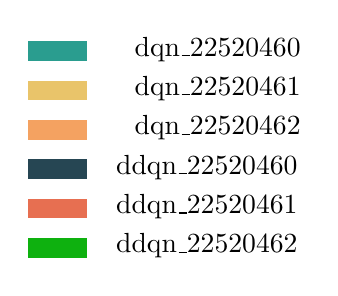
\begin{tikzpicture}
    % Định nghĩa các màu
    \definecolor{color1}{RGB}{38,70,83} % Màu #264653
    \definecolor{color2}{RGB}{42,157,143} % Màu #2a9d8f
    \definecolor{color3}{RGB}{233,196,106} % Màu #e9c46a
    \definecolor{color4}{RGB}{14,177,15} % Màu #0eb10f
    \definecolor{color5}{RGB}{231,111,81} % Màu #e76f51
    \definecolor{color6}{RGB}{244,162,97} % Màu #f4a261

    % Hình chữ nhật màu #2a9d8f (dqn_22520460)
    \fill[color2] (0,0) rectangle (0.75,0.25); % Tô màu #2a9d8f
    \node[right] at (1,0.15) {\vspace{5.0 mm} \vspace{5.0 mm} \vspace{1.0 mm}  dqn\_22520460};

    % Hình chữ nhật màu #e9c46a (dqn_22520461)
    \fill[color3] (0,-0.5) rectangle (0.75,-0.25); % Tô màu #e9c46a
    \node[right] at (1,-0.35) {\vspace{5.0 mm} \vspace{5.0 mm} \vspace{1.0 mm}  dqn\_22520461};

    % Hình chữ nhật màu #0eb10f (dqn_22520462)
    \fill[color6] (0,-1) rectangle (0.75,-0.75); % Tô màu #0eb10f
    \node[right] at (1,-0.85) {\vspace{5.0 mm} \vspace{5.0 mm} \vspace{1.0 mm}  dqn\_22520462};

    % Hình chữ nhật màu #264653 (ddqn_22520460)
    \fill[color1] (0,-1.5) rectangle (0.75,-1.25); % Tô màu #264653
    \node[right] at (1,-1.35) {ddqn\_22520460};

    % Hình chữ nhật màu #e76f51 (ddqn_22520461)
    \fill[color5] (0,-2) rectangle (0.75,-1.75); % Tô màu #e76f51
    \node[right] at (1,-1.85) {ddqn\_22520461};

    % Hình chữ nhật màu #f4a261 (ddqn_22520462)
    \fill[color4] (0,-2.5) rectangle (0.75,-2.25); % Tô màu #f4a261
    \node[right] at (1,-2.35) {ddqn\_22520462};
\end{tikzpicture}
\end{center}

\newpage
\subsection*{2.1. CartPole-v0}\addcontentsline{toc}{subsection}{2.1. CartPole-v0}

\begin{figure}[h!]
    % Hình ảnh thứ nhất
    \begin{minipage}{0.5\textwidth}

        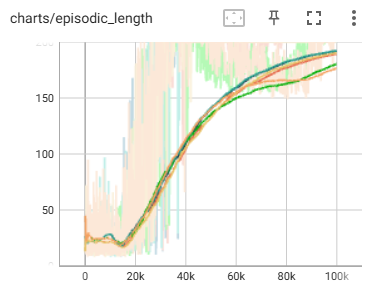
\includegraphics[width=7cm]{episodic_length_cartpole.png} 
        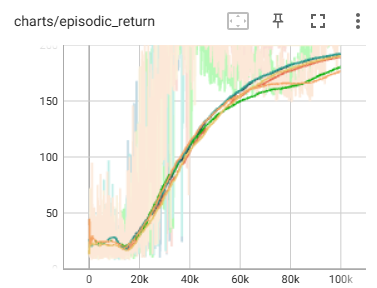
\includegraphics[width=7cm]{episodic_return_cartpole.png}
        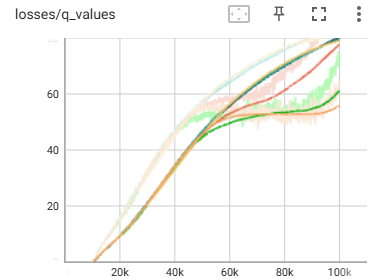
\includegraphics[width=7cm]{q_values_cartpole.png}
        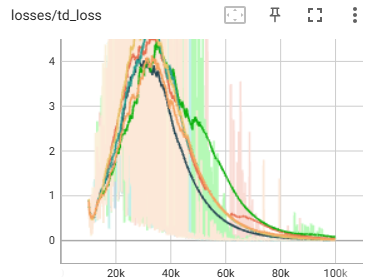
\includegraphics[width=7cm]{td_loss_cartpole.png}
        \caption*{\textbf{Figure 1.} CartPole-v0}
    \end{minipage}%
    \begin{minipage}{0.5\textwidth}
        \hspace*{5mm}In CartPole-v0, both DQN and Double DQN achieve nearly the same performance across all seeds, with the best episodes lasting 4 seconds because, in version v0 of CartPole, the episodes are truncated when the episode length exceeds 200$^{[1]}$.
        \\
        \hspace*{5mm}In the two plots of \textbf{episodic\_length} and \textbf{episodic\_return}, for each seed, the algorithms exhibit nearly overlapping lines and consistently achieve the maximum result of 200 in this environment. The \textbf{td\_loss} in all experiments converges to 0. However, in the \textbf{q\_values} plot, at seed 22520461, we observe that the \textbf{q\_values} of DQN are higher than those of Double DQN. This could indicate that DQN suffers from overestimation bias. However, this phenomenon is not observed with other seeds, and eventually, the \textbf{q\_values} of both algorithms converge for this seed as well. Ultimately, this environment cannot effectively assess the overestimation bias issue, as CartPole-v0 is considered relatively simple, with a small state and action space. In more complex environments, the differences between DQN and Double DQN regarding overestimation bias may become more apparent, such as in BreakoutNoFrameskip-v4.

        \begin{center}
            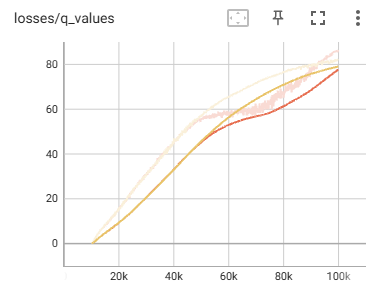
\includegraphics[width=7cm]{q_values_cartpole_22520461.png}
            \caption*{\footnotesize \textbf{Figure 2.} CartPole-v0 with seed=22520461} % Định dạng chữ nhỏ hơn trong caption
        \end{center}
        \footnotesize [1]: \href{https://www.gymlibrary.dev/environments/classic_control/cart_pole/}{CartPole-Gym Documentation}
    \end{minipage}
\end{figure}
\newpage
\subsection*{2.2. BreakoutNoFrameskip-v4}\addcontentsline{toc}{subsection}{2.2. BreakoutNoFrameskip-v4}
\begin{figure}[h!]
    % Hình ảnh thứ nhất
    \begin{minipage}{0.5\textwidth}

        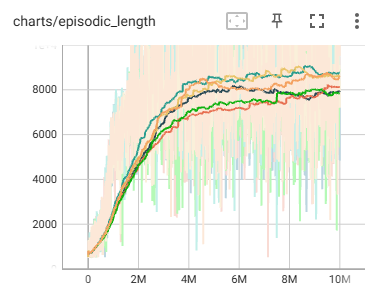
\includegraphics[width=7cm]{episodic_length_breakout.png} 
        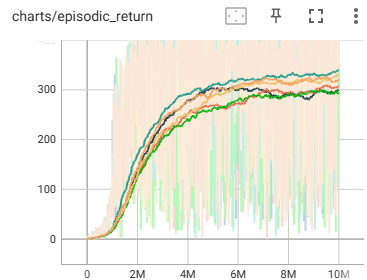
\includegraphics[width=7cm]{episodic_return_breakout.png}
        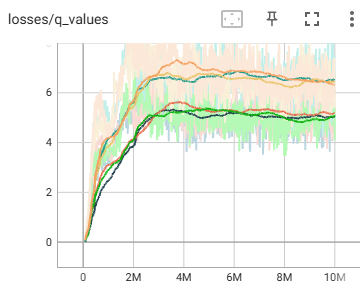
\includegraphics[width=7cm]{q_values_breakout.png}
        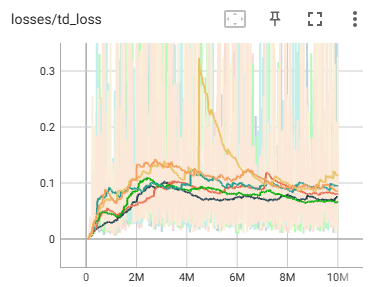
\includegraphics[width=7cm]{td_loss_breakout.png}
        \caption*{\textbf{Figure 3.} BreakoutNoFrameskip-v4}
    \end{minipage}%
    \begin{minipage}{0.5\textwidth}
        \hspace*{5mm}In the BreakoutNoFrameskip-v4 environment, the differences between DQN and Double DQN become more evident. In all three plots \textbf{episodic\_length}, \textbf{episodic\_return}, and \textbf{q\_values}, Double DQN consistently shows lower curves compared to DQN. The fact that Double DQN has more stable and lower \textbf{q\_values} demonstrates that DQN suffers from overestimation bias in this environment. This is further supported by the observation that the \textbf{td\_loss} of DQN is always higher than that of Double DQN, particularly at seed 22520461, where the \textbf{td\_loss} is significantly higher in the \textbf{global\_steps} range of 4M to 6M compared to other curves. The output videos also illustrate the stability of Double DQN and its superior performance over DQN.
        \\
        \hspace*{5mm} As mentioned in the introduction, the difference between DQN and Double DQN lies in the fact that Double DQN is effective at reducing the overestimation of Q-values and improving the stability of learning. This is achieved by separating the processes instead of using a single network to both select the best action and estimate its Q-value. One network selects the best action (based on current Q-values), while another network is used to estimate the Q-value corresponding to that action.
        \begin{center}
                \begin{tabular}{|c|c|}
                \hline
                \textbf{Algo\_Seed} & \textbf{Max Score} \\
                \hline
                ddqn\_22520460 & 420 \\
                ddqn\_22520461 & 411 \\
                ddqn\_22520462 & 420 \\
                dqn\_22520460  & 411 \\
                dqn\_22520461  & 391 \\
                dqn\_22520462  & 394 \\
                \hline
                \end{tabular}
                \caption*{\footnotesize \textbf{Table 1.} Best Score in BreakoutNoFrameskip-v4}
        \end{center}

    \end{minipage}
\end{figure}
\section*{3. Conclusion}
\addcontentsline{toc}{section}{3. Conclusion}
\hspace*{5mm} All the algorithms and seed i runned with this tempalte command:
\begin{minted}[bgcolor=LightGray, fontsize=\footnotesize]{Python}
python cleanrl/algo.py --seed seed --env-id game --total-timesteps num_steps --capture_video
\end{minted}
\vspace*{-10mm}
\begin{itemize}
    \item If game is 'CartPole-v0' the nums\_steps will be 100000.
    \item If game is 'BreakoutNoFrameskip-v4' the nums\_steps will be 10000000.
\end{itemize}   
\hspace*{5mm} The best videos of each algorithm in  environments is stored in this \href{https://drive.google.com/drive/u/1/folders/1Vw7R7SNeh44s3hq5KQ8unOkwG5vIrs0W}{link}.
\\
\hspace*{5mm} Additionally, other studies have also found that DDQN can lead to improved performance on tasks such as playing the card game Hanabi, controlling a simulated robot arm, and navigating a simulated 3D environment. In general, DDQN has been found to be particularly effective at reducing the overestimation of the Q values and improving the stability of learning.
\\
\hspace*{5mm}However, Double DQN is not a Panacea and may not always lead to improved performance. In fact, some studies have found that DDQN can perform worse than traditional DQN on certain tasks, such as playing the game of Go. Therefore, it is important to carefully evaluate the performance of DDQN on each specific task to determine whether it is likely to be beneficial. A comprehensive list of results performed by the authors of the DDQN paper is available on page 10 of the \href{https://arxiv.org/pdf/1509.06461}{paper}.
\\
\hspace*{5mm}In summary, DDQN has been shown to improve performance on many reinforcement learning tasks, but it is not always the best choice and its effectiveness can vary depending on the specific task$^{[2]}$.
\begin{flushright}
\scriptsize [2]: \href{https://dilithjay.com/blog/ddqn}{Double Deep Q-Networks (DDQN) - A Quick Intro (with Code)}
\end{flushright}


\end{document}
